\documentclass[12pt,letterpaper]{report}
\usepackage{graphicx}
\usepackage{scrextend}
\usepackage{vmargin}
\usepackage{graphicx}
\usepackage{multirow}
\usepackage[utf8]{inputenc}
\usepackage[spanish]{babel}
\usepackage{multicol}
\usepackage{enumerate}
\usepackage{float}
\usepackage{amsmath, amsthm, amssymb, amsfonts}
\usepackage[usenames]{color}
\parindent=0mm
\pagestyle{empty}
\definecolor{miorange}{rgb}{0.91, 0.43, 0.0}
\begin{document}
\setmargins{2.5cm}      
{1.5cm}                     
{2cm}  
{24cm}                    
{10pt}                          
{1cm}                          
{0pt}                             
{2cm}
\begin{flushright}
\today
\end{flushright}
\vspace{-1.75cm}
\section*{Tarea Clase 12}
\subsubsection*{Calcular el valor de x de cada figura utilizando las razones trigonométricas vistas:}
\begin{figure}[H]
\centering
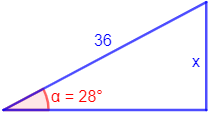
\includegraphics[scale=1]{P1.png}
\caption{Problema}
\end{figure}
\begin{figure}[H]
\centering
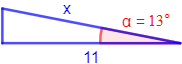
\includegraphics[scale=1]{P2.png}
\caption{Problema}
\end{figure}
\begin{figure}[H]
\centering
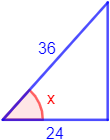
\includegraphics[scale=1]{P3.png}
\caption{Problema}
\end{figure}
\begin{figure}[H]
\centering
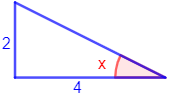
\includegraphics[scale=1]{P4.png}
\caption{Problema}
\end{figure}
\begin{figure}[H]
\centering
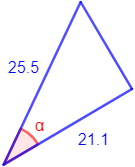
\includegraphics[scale=1]{P5.png}
\caption{Problema}
\end{figure}
\begin{figure}[H]
\centering
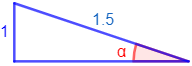
\includegraphics[scale=1]{P6.png}
\caption{Problema}
\end{figure}
\begin{figure}[H]
\centering
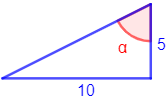
\includegraphics[scale=1]{P7.png}
\caption{Problema}
\end{figure}
\begin{figure}[H]
\centering
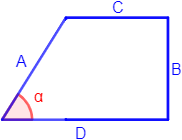
\includegraphics[scale=1]{P8.png}
\caption{Problema}
Calcular el área donde $\alpha=58$, B=C, A=24.6
\end{figure}
\end{document}